

\section{Electricity price forecasting} \label{sec:electricity_price_forecasting}

A lot of research has been going on in electricity price forecasting in power markets. Different strategies and models have been developed of which the most relevant regarding this thesis will be discussed. 


\subsection{Forecasting spot electricity prices with time series models}

In \cite{weron2005forecasting} the authors state that forecasting electricity prices with accuracy levels comparable to electricity load forecasting is hard to achieve, as different seasonality patterns (e.g.~daily, weekly, annually) and exogenous variables (such as loads and network constraints) have to be taken into account. 

%See also "`Forecasting electricity prices"' pg. 6, 19 ...

Three basic types of models for electricity price forecasting have been identified \cite{bunn2003forecasting,weron2005forecasting}: 

\begin{itemize}
	\item parsimonious stochastic models
	\item structural or fundamental models
	\item non-parametric models
\end{itemize}

The first class of models aims to capture the data's statistical characteristics and extrapolate these patterns into the future. Energy price characteristics such as mean reversion and price spikes are modeled to more accurately resemble the actual price time series. Structural or fundamental models take a different approach as they take into account external factors (fundamentals) such as load or weather data combined with historical price series to derive accurate forecasts. As the name implies, non-parametric models do not depend on parameter estimations and properties of the time series but define complex algorithms to map input variables to outputs that represent electricity price forecasts for a specific period of time. 
%their goal is to understand market performance and the rich structure of electricity prices thereby combining historic market prices and fundamentals such as load, weather and plant data \cite{bunn2003forecasting}. 
%where focus has been laid on a combination of the first two types of models. 

In \cite{weron2005forecasting} forecast models are developed to model the next 24 hours of the following day (day ahead) by utilizing historical prices and demand as well as day ahead load predictions. In order to model the daily variation of demand, costs and operational constraint models have been built for each hour separately which is inspired by studies of demand forecasting \cite{bunn2000forecasting}. 

Data was taken from the Californian power market from before and during the market crash in 2001 \cite{weron2005forecasting}. Preprocessing has been done by removing outliers (substitution by the arithmetic average of neighbouring values), mean removal (center data around zero) and logarithmic transformations of load ($z_t = \log(Z_t)$) and price ($p_t = \log(P_t)$) time series. The latter approach is used to obtain a more stable variance of the time series data. 

To achieve seasonal autoregression models the log price $p_t$ was made dependent on the same hour in previous days and weeks as well as on an aggregate function based on the previous day prices. The system load has been used as the fundamental variable as strong correlations between loads and prices have been revealed (Figure \ref{fig:log_loads_vs_log_prices}). 

\begin{figure}[htbp]
	\centering
		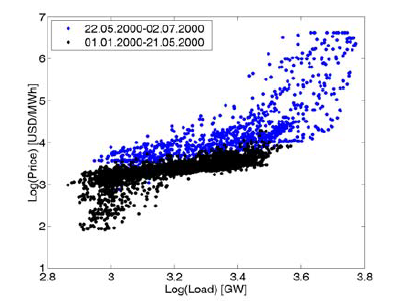
\includegraphics{figures/state_of_the_art/log_loads_vs_log_prices.PNG}
	\caption{The dependence between the
hourly log prices and hourly log system
loads in California for the period January 1
– July 2, 2000. \cite{weron2005forecasting}}
	\label{fig:log_loads_vs_log_prices}
\end{figure}

As can be observed the dependence between loads and energy prices is almost linear except for very low and very high loads, where electricity prices tend to jump to lower and higher values, respectively. 

Results show that for the proposed dataset ARX models (AR with exogenous variables) exhibit lower mean weekly errors (MWE) than AR models which in turn had significantly lower errors than standard ARIMA models. The difference is the separate modeling of individual hours for the ARX and AR models as opposed to an 48 hour aggregate modeling for ARIMA models. 

\subsection{ARIMA models to predict next-day electricity prices}

The authors in \cite{contreras2003arima} propose the application of ARIMA models for day ahead energy price forecasting based on data in the Spanish and Californian power markets. These models are based on time series analysis and results show that accurate electricity price forecasting for the aforementioned power markets is possible. Depending on the market and selected time range average weekly prediction errors 
range from 5\% to 10\%. These results are quite reasonable given that prices from the Californian market in the year 2000 have been selected which has been a very volatile and unstable time period due to the market crash in early 2001 \cite{weron2007modeling}. 

The described model generation process consists of five steps: 

\begin{itemize}
	\item[0)] A class of models is formulated assuming certain hypotheses.
	\item[1)] A model is identified for the observed data.
	\item[2)] The model parameters are estimated.
	\item[3)] If the hypotheses of the model are validated, go to Step 4, otherwise go to Step 1 to refine the model.
	\item[4)] The model is ready for forecasting.
\end{itemize}

This process is taken from the Box Jenkins methodology for forecast model generation \cite{hibon1997arma}.

Interestingly only five hour training periods are needed to model forecasts for the next consecutive hour for Spanish power prices, only two hour training periods are needed for modeling Californian energy prices. 
Through outlier detection the resulting forecasts could have been slightly improved but as stated in \cite{contreras2003arima} this would result in significantly increased computation time. 

%The first step (0) consists of determining a suitable class of models that can be applied to the time series based on observed characteristics, e.g.~high frequency, nonconstant mean and variance, and multiple seasonality. The hypothesis of the model at this step assumes a forecast error term with a normal distribution having a zero mean and constant variance. 
%
%In step 1) a trial model has to be selected for which data has to be made stationary. Through application of a logarithmic transformation a more stable variance can be achieved whereas (seasonal) differencing of data may result in a more stable mean. In order to find appropriate autoregressive and moving average coefficients for the resulting ARIMA model autocorrelation (ACF) and partial autocorrelation (PACF) plots may be consulted to retrieve a first fit of the model. 
%
%Step 2) consists of estimation of parameters which is typically done by applying the maximum likelihood function with respect to the parameters. In order to optimize forecasting performance outlier detection methods may be applied to minimize the impact of single "`spikes"' in the data. 
%
%In step 3) the residuals (forecast errors) of the resulting model are evaluated based on desired characteristics. Residuals should exhibit zero mean, constant variance, should follow a normal distribution and should be uncorrelated. Suitable tests for these properties are portmanteau tests (Ljung box, Box Pierce) and examination of ACF and PACF plots to find dependencies within the data. 
%
%Step 4) is concluding the model selection process. The resulting model of step 2) is used for forecasting based on trained data. 




\subsection{Classification of forecast models applicable to electricity price forecasting}

Electricity price forecast models in general can be classified in three different sets of models: game theory models, time series models and production cost or simulation models \cite{gonzalez2005modeling, aggarwal2009electricity} (Figure \ref{fig:classification_of_price_forecasting_models}).  

Game theoretic models study the evolution of energy prices by analyzing the strategic behavior of the agents \cite{gonzalez2005modeling}. They aim to model the strategies of market participants (agents) as formalized games and identify solutions to those games \cite{aggarwal2009electricity}. Specifically equilibrium models analyze the strategic market equilibrium which describes the set of strategies such that no player in the market can improve its position if its rivals maintain their strategies \cite{gonzalez2005modeling}. 

\begin{figure}[htbp]
	\centering
		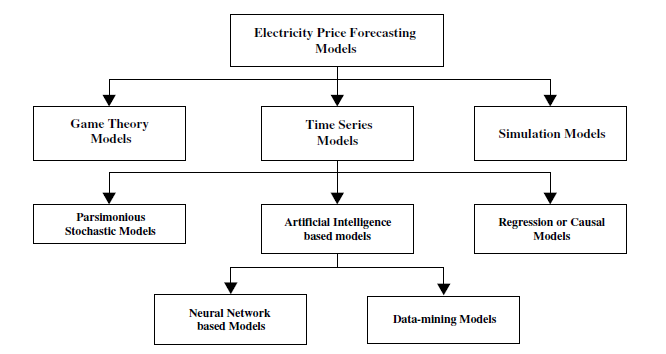
\includegraphics{figures/state_of_the_art/classification_of_price_forecasting_models.PNG}
	\caption{Taxonomy of price forecasting models \cite{aggarwal2009electricity}}
	\label{fig:classification_of_price_forecasting_models}
\end{figure}

Production cost or simulation models build an exact model of the system and emulate the underlying process \cite{aggarwal2009electricity}. 
They simulate the operation of power systems as well as agents' strategic behavior impact on market prices \cite{gonzalez2005modeling,lora2007electricity}. Based on the system model mathematical models are generated by the simulation method which are then solved for price forecasting. 
Due to their advanced modeling of the system these models require detailed system operation data and exhibit high computational costs \cite{aggarwal2009electricity}. 

Time series models on the other hand are based on historical price data and statistically model price evolution but do not model the underlying system's behavior in detail. Time series models have the advantage to exhibit a simpler structure and require less information than production cost models or game theory based models \cite{lora2007electricity}. A range of different types of time series models is available, from "`black box"' models that are only based on historical price data to complex structural models that include various explanatory variables (e.g.~load demand or fuel prices). 

Time series models can in turn be classified into classical time series models and models based on machine learning techniques \cite{lora2007electricity}. The benefit of classical time series models is that they exhibit a less complex structure and therefore less computation time than machine learning based models. However it can be harder to obtain accurate forecasts for non-linear time series such as energy prices \cite{lora2007electricity}. 

Parsimonious stochastic models are inspired by financial research to model characteristics of energy prices. Stochastic models are either based on stationary or non-stationary time series \cite{gonzalez2005modeling}. Stationary denotes the characteristic of a time series to exhibit zero mean and constant variance \cite{hyndman2012forecasting}. The first type of models can only be based on stationary time series (e.g.~AR, MA and ARMA models). The latter type can handle non-stationarity by transforming data to a stationary series within the model generation process (e.g.~ARIMA, GARCH models) \cite{hyndman2012forecasting, aggarwal2009electricity}. 

Regression or casual models handle the relationship between a dependent variable (electricity price) and a number of independent variables (e.g. load or weather conditions). By evaluating the correlations between independent and dependent variables the explanatory variables for the model can be identified \cite{aggarwal2009electricity}. 

Finally artificial intelligence based methods can be divided into neural network based models and data mining models \cite{aggarwal2009electricity}. 
Both of these types of models can be used to discover non-linear relationships that might be difficult to obtain by statistical models. By capturing the autocorrelation structure of the time series, neural network models extrapolate patterns discovered in historical price data into the future \cite{gonzalez2005modeling}. In constrast data mining methods use data mining techniques based on categorization of data, e.g.~Bayesian categorization or closest k-neighborhood categorization \cite{aggarwal2009electricity}. 


%Regarding machine learning approaches, artificial neural networks (ANN) have been studied extensively in relation to electricity price forecasting \cite{vahidinasab2008day, singhal2011electricity, pao2007forecasting, amjady2006day, catalao2007short, 
%gareta2006forecasting, duanelectricity, szkuta1999electricity}. Neural network models are trained to model non-linear relationships between applicable input variables and historical energy prices. 

%Statistical time series models as well as artificial intelligence based models have been researched extensively. 

When comparing statistical time series models with neural network based models a number of benefits and drawbacks can be discovered related to energy price forecasting. 

Extensive research has been made regarding stochastic time series models whereby models may be applied to single \cite{garcia2005garch, weron2008forecastingWh, weron2008forecasting, nogales2002forecasting, cuaresma2004forecasting, tan2010day, conejo2005day} or complex multiple seasonality patterns \cite{de2011forecasting, gould2008forecasting, zivot2003vector}. 
Studies show that univariate time series models may be improved significantly by modeling each hour of the day separately \cite{cuaresma2004forecasting, weron2008forecasting}. However this requires model building separately for each hour which increases the amount of effort needed especially in dynamic forecasting environments. 
It is also stated that inclusion of non-linear phenomena would drastically increase computation time for time series models \cite{cuaresma2004forecasting}. 


%Game theoretic model approaches for electricity markets with tight \cite{hu2008game,gan2005auction} and weak \cite{gan2005auction} capacity constraints have been developed. 
%models may be classified in two types: univariate and multivariate time series models. 
Regarding machine learning approaches, artificial neural networks (ANN) have been studied extensively in relation to electricity price forecasting \cite{vahidinasab2008day, singhal2011electricity, pao2007forecasting, amjady2006day, catalao2007short, 
gareta2006forecasting, duanelectricity, szkuta1999electricity}. 
Results show that ANN models have the potential to outperform statistical models such as Autoregressive (AR) or Autoregressive Integrated Moving Average (ARIMA) models \cite{pao2007forecasting, catalao2007short}. This may be due to their ability to more accurately model the underlying system behavior while they excel at modeling non-linear relationships in the dataset. 

However, in order to successfully apply forecasting based on neural network models a set of requirements have to be met \cite{catalao2007short}: Availability of sufficient amounts of data, adequate selection of input/output samples, an appropriate number of hidden units and sufficient computational resources. In case these requirements can not be met or it is not possible to appropriately parametrize the model statistical models provide a good alternative for modeling energy prices. 




\section{Cost optimization in geo distributed data centers}

\subsection{A Study of Electricity Price Features on Distributed Internet Data Centers}

A comprehensive study about optimization of energy costs under different operational and energy cost prediction regimes is presented in \cite{de2013study}. 

The focus of that paper is to leverage price differences across different energy markets in a network of geo distributed data centers to minimize energy costs by migrating resources to currently cheaper locations. It takes into account the impact of several metrics including the level of price variability, time lag between locations, reconfiguration delay and accuracy of energy price predictions. 

To provide a forecasting model based on the given data the Box-Jenkins method is used to build an ARIMA model characterizing the underlying electricity price data:

\[ ARMA(p,q) : P_t = \epsilon_t + \sum_{i=1}^{p}{\phi_i P_{t-i}} + \sum_{j=1}^{q}{\theta_j \epsilon_{t-j}}\] 

where $p$ and $q$ are the number of autoregressive and moving average terms, $\phi_i$ and $\theta_j$ denote the model coefficients and $\epsilon_t$ denotes the error term at time $t$. To accurately model seasonality in the data an $SARIMA(p,d,q)(P,D,Q)[s]$ model has been used which includes the number of terms $p,q$ and $P,Q$ as non-seasonal and seasonal parameters and $d$ and $D$ for non-seasonal and seasonal differencing, respectively. 

Price time series have been generated with different levels of variability $\sigma_{Price}^{2} \in \{50, 126.6, \ab 300, 500\}$. In addition, prediction errors have been used to simulate different forecast accuracy levels, $\sigma_{pred} \in \{2.0, 5.0, 10.0\}$. 

Thus, $P = \{p_1,\ldots,p_T \}$ denotes a price time series and $\hat{P} = \{\hat{p_1},\ldots,\hat{p_T}\}$ a simulation of forecast values such that 
$\hat{P_t} = \mathcal{N}(P_t, \sigma_{pred}), \forall t \in T$. As a measure of accuracy the mean squared error (MSE) has been used: 
$MSE(P,\hat{P}) = \frac{1}{T} \sum_{t \in T}{(P_t - \hat{P_t})^2}$. 

The decision of workload assignment at a particular time $t$ is based on the number of active servers at location $i$ and the corresponding forecast prices $\hat{P_i}(t)$. The total cost at any given moment is defined by $\hat{C_t} = \sum_{i=1}^{N}{m_i \times \hat{P_i}(t) \times Po_i}$ where $Po_i$ denotes the power used by a server running at location $i$ and $m_i$ defines the number of running servers at location $i$. 

Results for different metrics achieved different cost savings \cite{de2013study}. When the number of locations involved in the simulation is increased, cost savings up to 10\% have been reported when going from 1 up to 20 locations. The more locations are considered the greater benefit can be drawn from price differences and time lags between different locations. 

Price variability has been simulated with $\sigma_{price}^{2} \in \{0,5,\ldots,500\}$ and resulting costs have been estimated. It was shown that up to 15\% of savings could be achieved when comparing the maximum and minimum simulated price variabilities. 

Concerning time lags it is stated that the most benefit could be drawn from locations in timezones that are sufficiently distant from each other due to the daily seasonality observed in energy prices. For this scenario up to 15\% cost savings have been achieved for locations that were perfectly "`out of phase"'. 

Finally results show that forecast errors have a major impact on resulting costs. In order to quantitatively measure the impact of forecast deviations $\sigma_{pred}$ has been increased stepwise in the range $0,\ldots,5$ by steps of $0.1$.
The resulting MSE is quadratically rising with the level of $\sigma_{pred}$, thus when errors are at maximum a 10\% revenue loss is expected. 
Therefore accurate forecasts are very important to achieve major cost savings in a multi cloud environment. 




\subsection{Cutting Down the Energy Cost of Geographically Distributed Cloud Data Centers}

This paper aims to minimize energy costs in geographically distributed data centers by taking into account spatio-temporal variation in electricity prices and the outside weather temperature \cite{guler2013cutting}. The scenario is modeled as a linear programming problem which is solved by presenting various heuristic solutions to the problem. 

While providing algorithms for minizing energy costs resulting SLA penalties as well as cooling related costs are taken into account. 
For each data center a performance coefficient (CoP) is calculated which is based on outside weather temperature where the coefficient increases linearly with rising temperature. A data center may have different types of servers exhibiting different performance metrics and capacities. 

Energy costs are calculated as the sum of server power consumption over a specific time range multiplied by the applicable energy prices during that time. 
The total costs for data center $i$ are defined as $E_{i}^{total} = E_{i}^{IT} \times CoP(T_i)$ where $T_i$ denotes the temperature at location $i$. 

The actual time a job $j$ needs when running on a type $k$ server $s$ is defined as 
\[  T_{j,s} = \frac{c_j \times f_j \times l_j}{c_k \times f_k}  \] 
where $c$ and $f$ denote the number of cores and frequency available / needed by a server / job and $l$ denotes the expected runtime of job $j$. 
A penalty occurs if the total runtime of a job exceeds the expected runtime when running on server $s$. 

The goal is to minimize the sum of total energy and penalty costs over all data centers 
\[ \min \sum_{i=1}^{N}{E_{i}^{total} + Pen_i} \]
where $Pen_i$ denotes the total penalty cost for data center $i$. 

Based on the proposed linear optimization problem two types of scheduling algorithms are introduced, immediate and delayed. Immediate scheduling algorithms are defined as CheapestDC and CheapestS where the former places resources randomly on hosts located at the currently cheapest data center while the latter includes outside weather temperature as well in the calculation. Delayed scheduling algorithms additionally consider historical energy prices to decide whether jobs should be delayed to a future time stamp. 

Simulation runs over six data centers at different locations handling three types of workloads were conducted to evaluate different scheduling algorithms.
Results show that delayed scheduling techniques on light workloads achieve over 5\% on overall cost savings compared to the baseline random scheduler. Also, spatial electricity price variations have the most impact on cost savings followed by temporal electricity price changes and reduced cooling costs due to outside weather temperature. 


\subsection{Studies for cost optimizations in multi-electricity-market environments}

Different studies have been developed for optimizing energy costs in multi market environments. 

In \cite{buchbinder2011online} the basic tradeoff between energy and bandwidth costs is discussed for migrating virtual machines between geographically distributed data centers. 
Three different algorithms have been evaluated on a set of 30 US locations covering three years of next day electricity data. Out of the two greedy algorithms and the online migration algorithm the latter provided the best results with only 4 to 6 \% off the optimal offline solution. 

The authors in \cite{rao2010minimizing} aim to minimize energy costs while guaranteeing quality of service by referring to a constrained mixed integer programming model. The approximated linear programming model is converted to a minimum cost flow problem which can be solved fast and efficiently. With five frontend web portal servers targeting three internet data centers cost reductions up to 30\% are achieved within the simulation. 

An extensive study on electricity price features and its implications for existing cloud systems is given in \cite{qureshi2009cutting}. While taking into account server energy elasticity and bandwidth constraints a maximum cost savings of 45\% could be achieved when running a simulation over 39 months including 29 locations. However, in order to achieve these results bandwidth constraints are relaxed and large distances to clients have to be permitted. 

A different approach is examined by \cite{simarro2011dynamic} where dynamic pricing schemes of different cloud providers are taken advantage of to reduce investment of users. The assumption is that prices for each cloud provider change according to demand and thus virtual cluster placements can be optimized across different cloud providers. As infrastructure is dynamically distributed without notice of the user it provides an efficient and convenient way of reducing costs for cloud users. 

Cost based multi cloud schedulers have been investigated in \cite{le2009cost} and \cite{tordsson2012cloud}. 
A cloud scheduler for simplified management of virtual machines has been developed in \cite{armstrong2010cloud}, a green cloud scheduler in \cite{lucanin2013take}. 
Also, schedulers based on genetic algorithms were proposed by \cite{dutta2011genetic} for cost based multi QoS optimizations and \cite{ge2010ga} for improving delay scheduling policy. 


%
%Active research topics in this field include electricity cost reduction in data centers \cite{guler2013cutting, le2011reducing}. A comparison of different approaches considering spatial and temporal energy price changes and the contribution of the outside temperature to the resulting cooling effort and expense is outlined in \cite{guler2013cutting}. In \cite{le2011reducing} a set of homogenous data centers is simulated where the focus lies on the effects of changing workloads and migrations on the cooling infrastructure and on intelligent scheduling to reduce energy consumption and energy costs, respectively. 
%
%The authors in \cite{lucanin2013take} propose a green cloud approach using real time electricity prices where the duration and time of price peaks are estimated and VMs are paused during these times to reduce energy costs and save energy. Customers may choose between ``green'' and normal instances, taking into account some loss of availability for a reduced price. 
%
%
%
%In \cite{rao2010minimizing} a cloud consisting of several Internet Data Centers (IDC) is examined with regard to cost optimization which is done by intelligently assigning workload to data centers based on current energy prices. Two of these data centers in the scenario are connected to deregulated wholesale energy markets whereas the other one is connected to a regulated utility region charged by a fixed pricing scheme. Since price change differences in deregulated energy markets can be considerable energy cost reductions may be achieved by assigning workload based on changing energy prices.  %For the purpose of the simulation five front-end Web portal servers process a total workload of about $10^5$ requests per second. 
%
%In this paper the approaches of optimal and average workload assignments are visually and formally compared to gain insights into the total electricity cost reduction. The optimal workload assignment is calculated with respect to workload and delay constraints that are considered in a minimum cost flow problem based on a linear programming model. Thus the goal is to minimize costs without compromising quality of service constraints. 
%%The proposed cost reductions amount up to 30 percent for a single hour test within the given time range. 
%%The results measured at two timestamps at a specific day seem promising, since total cost reductions could be achieved by 30\% and 17\% respectively. 
%
%The differences compared to this work is that in \cite{rao2010minimizing} they do not consider longer running jobs as used in scientific calculations or large optimization problems that may take several hours to complete. Thus the impact of migrations is not examined in this scenario. In addition the possibility of energy price forecasting is not considered which may result in even greater energy cost reductions. 
%
%Another study on cost reductions in Internet Data Centers has been done where different aspects of cost reductions including cost prediction schemes have been considered \cite{de2013study}. Since up to 15\% of total capital investment is spend on energy related costs 
%%(paper references \cite{greenberg2008cost} - old, from 2009!!) 
%a special effort is invested to reduce the amount of energy costs through cost aware operations. %(TODO: Move to introduction?)
%
%In this paper cost optimization is seen as an assignment problem where an overall cost function is minimized through intelligent workload allocation. During the investigation different variables and their impact on resulting energy costs are considered which are price volatility, price predictions including variable prediction errors, time lag between locations and reconfiguration delays. 
%
%Similar to this work the simulation is run with the same set of fixed parameters to evaluate the impact of the various scenarios. It is observed that prediction errors greatly impact workload allocation where cost penalties due to non-optimal assignments increase quadratically with an increase of forecast errors \cite{de2013study}. Also with increasing number of locations the minimum cost of optimal assignments can be greatly reduced. Greater price volatility is beneficial as well since then price aware assignments will have greater impacts. 
%
%A comprehensive study on cost reductions and energy market characteristics in an environment where data centers are placed within the reach of different energy markets is presented at \cite{qureshi2009cutting}. Based on geotemporal variations of energy prices the maximum cost reductions under different scenarios are evaluated. Energy expenses are estimated for various large scale companies like Google and Yahoo to state the actual savings and the amount of reductions in energy costs that would be possible. 
%They also discuss the impact of considering bandwith constraints and maximum client server distances on cost reductions. 
%
%Interestingly enough long term seasonalities in the energy price data has been discovered that spanned multiple energy markets. This is an important fact when training forecasting models since predictions can become a lot more accurate. An important fact that was revealed about energy markets was that data from different energy markets was much less correlated than data from the same area. Thus to take full advantage of energy price differences data centers located at different energy markets should be combined \cite{qureshi2009cutting}. 
%
%With different state of the art energy models and simulation constraints a summary of possible cost reduction schemes was presented. However no migration or forecasting of energy price data has been done which could further improve scenarios with longer running jobs. In addition these cost reductions are only valid under specific assumptions that large cloud providers would need to implement such as connection to wholesale energy markets and reasonable server energy elasticity. 
%



\section{Optimize resource scheduling algorithms}

\subsection{A task scheduling algorithm based on load balancing in cloud computing}

In \cite{fang2010task} a two level scheduling model has been implemented (Figure \ref{fig:two_level_resource_scheduling}). 

\begin{figure}[htbp]
	\centering
		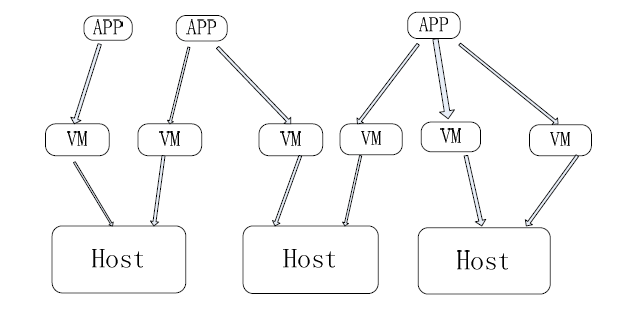
\includegraphics[width=0.7\textwidth]{figures/state_of_the_art/two_level_resource_scheduling.PNG}
	\caption{Two level scheduling model \cite{fang2010task}}
	\label{fig:two_level_resource_scheduling}
\end{figure}

A two stage process is described where the first scheduler creates the task description of a virtual machine s.t.~the task will have a perfect fit on a virtual machine whereas the second scheduler is responsible to find appropriate resources (hosts) for the provisioned virtual machine. Thus an optimized resource scheduling is presented with focus on load balancing among different clouds. 

Tasks have a defined structure where task $t_i$ out of the set of all Tasks $T$ is defined as 

\[t_i = \{tId, tRr, tSta, tData, tVmch, tVm\}\]

\begin{itemize}
	\item $tId$ is the task identification
	\item $tRr$ denotes the required resources
	\item $tSta$ describes the state of the task where $tSta = \{tFree,tAllo,tSche,tWait,tExec,tComp\}$
	\item $tData$ defines the relative data of the task (computational load, input and output data)
	\item $tVmch$ denotes the virtual machine specification where $tVmch = \{tId,tRr,tData\}$
	\item $tVm$ defines the assigned virtual machine of the task where $tVm = \{tId,thId\}$
\end{itemize}

Hosts on the other hand are defined as $h_j = \{hId, hTcap, hFcap, hData\}$, where

\begin{itemize}
	\item $hId$ denotes the host identification
	\item $hTcap$ is the total host capacity (set of resource capacities)
	\item $hFcap$ is the freely available host capacity
	\item $hData$ denotes the relative data of the host (including input and output bandwidth)
\end{itemize}

%Concerning the scheduling algorithm, the predicted task resource usage is defined as $VL_i$. 

The scheduling algorithm is based on the following equations: 

\[ HL_i = \frac{\sum_{j=1}^{n}{VL_j}}{n} \]

\[ avgl = \frac{\sum_{i=1}^{m}{HL_i}}{m} \]

\[ B = \frac{\sqrt{\sum_{i=1}^{m}{(HL_i - avgl)^2}}}{m} \]

where $VL_j$ is the predicted resource load for VM $j$, $HL_i$ is the average load for host $i$, $avgl$ denotes the average
load across all running hosts and $B$ denotes a metric for load balancing. 

The scheduler iterates over the set of hosts in each timestamp and determines the value of the load balancing metric $B$. In case the value of 
$B$ exceeds a predefined threshold $B_0$ or the predicted resource requirements for a virtual machine exceed the currently allocated resources 
the VM is migrated to a host occupying the least resources for optimal load balancing. 

Results show that considering dynamic resource requirements load is distributed across all machines leading to stable level of cloud utilization. 



\subsection{Efficient resource management for cloud computing environments}

In \cite{younge2010efficient} power aware and live migration scheduling techniques are proposed as a green cloud approach to increase overall system efficiency with minimal performance overhead. 

A new greedy based algorithm is presented to minimize power consumption. It is based on the findings that power consumption of a server does not increase linearly with the number of cores utilized. Instead, most power is drawn by one utilized core whereas power increases only slightly when comparing a server utilizing 7 to 8 cores. Thus a new VM scheduling algorithm is proposed that minimizes resulting power consumption within a data center. 

Hosts are assigned to a pool of resources where a pool can be initialized by a priority based evaluations system to either maximize performance or further minimize power consumption \cite{younge2010efficient}. Each VM request is checked against its resource requirements and available capacities in the pool and assigned to a host to maximize utilization and therefore minimize overall power consumption. 

In addition, live migration of virtual machines is applied to further optimize power consumption by shifting load away from under utilized hosts (Figure \ref{fig:server_power_consumption}). When load increases, Wake on Lan (WOL) technology is used to power servers back up again. Furthermore, a focus has been to reduce VM image size and boot time to optimize virtual machines for a server environment. 

%\begin{figure}[htbp]
	%\centering
		%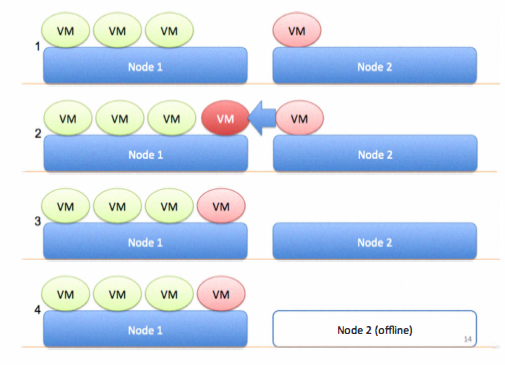
\includegraphics{figures/state_of_the_art/vm_migration_for_host_consolidation.PNG}
	%\caption{Virtual machine management dynamic shutdown technique \cite{younge2010efficient}}
	%\label{fig:vm_migration_for_host_consolidation}
%\end{figure}

\begin{figure}[htbp]
	\centering
		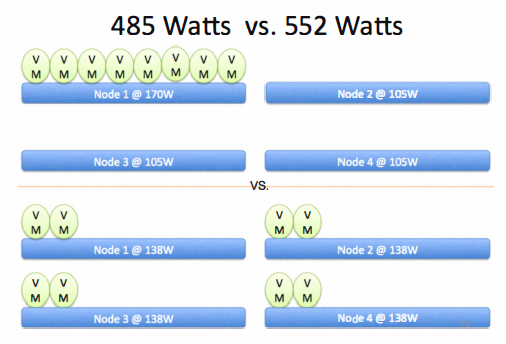
\includegraphics[width=0.7\textwidth]{figures/state_of_the_art/server_power_consumption.PNG}
	\caption{Illustration of scheduling power savings \cite{younge2010efficient}}
	\label{fig:server_power_consumption}
\end{figure}

Power aware resource scheduling has been simulated on an OpenNebula \cite{fontan2008opennebula} pool of 4 servers, equipped with 8 cores each. Power elasticity (power range from idle to peak power of a server) for this type of server is 61\% where a total reduction in power consumption of 12\% could be achieved. As the results are scalable also to large clusters significant power and cost savings are possible using the proposed approach. 


%
%
%
%\subsection{Server power management}
%
%A well known problem in power management is how to accurately and efficiently model a server's power consumption over time. At \cite{horvath2008multi} Horvath et al.~exploit dynamic voltage scaling (DVS) and multiple sleep states to reduce power consumption of a server cluster of about 23\% without significantly impacting performance. They propose that CPU utilization and frequency are the variables that have the most significant impact on the power consumption of a machine. This assumption is also used in other studies, e.g.~\cite{rao2010minimizing, hammadi2014survey, kliazovich2012greencloud}. 



\section{Virtual machine migration}
%\subsection{Virtual machine migration in cloud environments}


Live Virtual machine migration is defined as follows:
\begin{quote}
A source virtual machine (VM) hosted on a source server is
migrated to a destination VM on a destination server without
first powering down the source VM \cite{nelson2009virtual}.
\end{quote}

Thus efficient methods for transferring VM memory pages from the source to the destination host are needed which will be evaluated in the following sections. 
%One method is defined by resuming the destination VM before all memory pages from the source VM are transferred. This can be done by paging in any remaining VM memory pages from the source to the destination on demand. A second approach executes a pre-copy phase where memory is transferred in several rounds from the source to the destination host before launching the destination VM. Dirtied memory pages are re-transferred which have been dirtied during previous transfers of memory to ensure a consistent VM memory image at the destination. 
%
%The non-memory state of the VM is preferably available in a shared storage arrangement accessible by both the source and destination VMs such that it is only required to re-map the source VM's virtual disk to the destination VM. In case no shared storage is available, the source VM's non-memory state has to be transferred to the destination VM before or after the migration depending on the implementation. 


\subsection{Live migration of virtual machines}

In \cite{clark2005live} an efficient approach for live migration of virtual machines is presented. This paper targets the migration of entire OS within a virtual machine without noticeable service interruption. 

The applied method for migration should minimize both downtime and total migration time for the virtual machine. The first metric denotes the actual downtime of the VM where it is completely suspended and unaccessible to users. The second metric is defined by the total time between the start of the migration process until its end \cite{clark2005live}. 

Three methods have been identified that have been used previously. The \textit{pure stop-and-copy} approach halts the source VM, copies all memory pages to the destination host and resumes execution at the destination. Both downtime and total migration time are proportional to the amount of memory to be transferred which can lead to unacceptable downtimes. 

The \textit{pure demand migration} method is defined where essential data for running the VM is transferred to the destination host after which the destination VM is booted. Any missing memory pages create page faults and trigger a synchronous transfer from the source host on first use. This leads to poor performance until a sufficient amount of memory pages have been transferred. 

The \textit{pre-copy} approach combines an iterative push-phase with a very short stop-and-copy phase to minimize downtime. Any pages dirtied during a transfer of memory are re-sent in the next iteration until a sufficient amount of memory pages have been transferred to the destination host. In a final stop-and-copy phase the VM is suspended on the source host, remaining memory pages are copied to the destination and the VM is resumed at the destination. 

An important efficiency measure for VM migrations has been identified as the writable working set (WWS) \cite{clark2005live}. It is defined as a set of memory pages that are updated very frequently such that it is not worth keeping them consistent at the source and destination hosts. These set of pages should be copied only in the final stop-and-copy phase. An accurate measure of the WWS for the SPEC CINT2000 benchmark is depicted in Figure \ref{fig:tracking_writable_working_set}. 

In this graph the number of 4KB pages of memory dirtied within a corresponding 8 second interval are shown for each of the programs run in the benchmark. 
It is clearly visible that the number of pages contained within a WWS depends greatly on the behavior of the selected program. Workloads exhibiting a high amount of frequently updated pages such as \textit{gap} will provide only a small number of pages sensible for inclusion in a pre-copying phase. 
Thus the downtime and cost resulting from a VM migration depends to a great extent on the type of workload being migrated and the exact moment of the start of the migration. 

%Thus the source virtual machine does not hold any dependencies related to the destination VM after migration has finished. The in-memory state of the VM is transferred efficiently such that a seamless live migration becomes possible. 


\begin{figure}
	\centering
		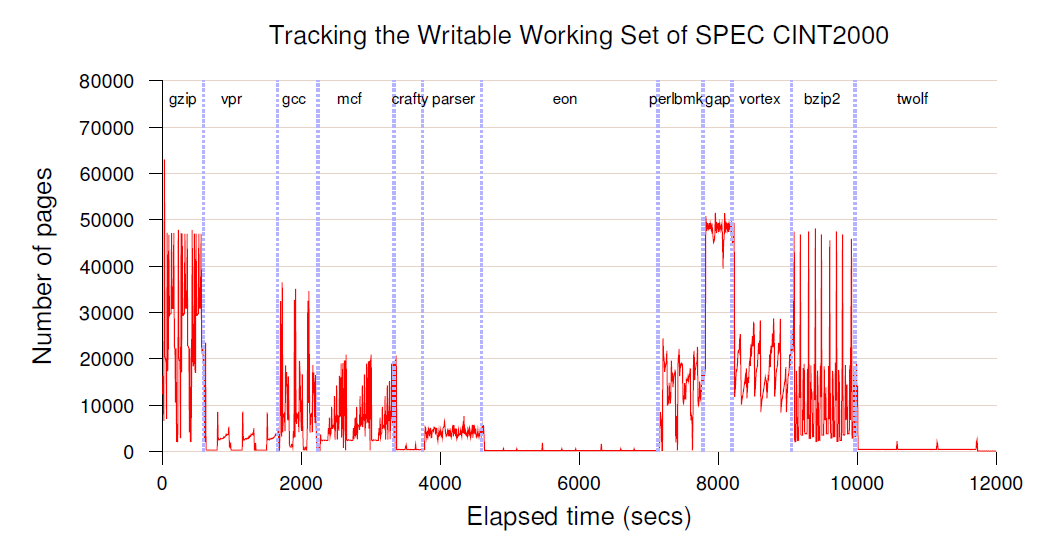
\includegraphics[width=0.94\textwidth]{figures/state_of_the_art/tracking_writable_working_set.PNG}
	\caption{WWS curve for a complete run of SPEC CINT2000 (512MB VM) \cite{clark2005live}}
	\label{fig:tracking_writable_working_set}
\end{figure}



Results for different kind of workloads indicate that even in the worst case the pre-copy approach significantly reduces downtime compared to the stop-and-copy method. As bandwidth has a direct impact on migration downtime performance can be further increased by raising the bandwidth assigned to the VM migration. 

Migration downtimes have been evaluated for different sized VMs running various kinds of workloads. Resulting downtimes range from only 60 ms for small sized VMs (64 MB) and low dirty page rate to 3.5 seconds for large VMs (512 MB) with frequently updated dirty page rates. It is stated that realistic workloads can be migrated with a downtime as low as 210 ms in a virtualized cluster environment. 


\subsection{Performance and energy modeling for live Migration of Virtual Machines}

A thorough evaluation of migration performance and resulting migration costs is given by \cite{liu2013performance}. 

The authors provide methods to quantitatively predict migration performance and resulting energy cost. A refined pre-copy approach is used to efficiently transfer memory pages in iterative rounds where in each round the memory pages dirtied in the previous round are re-sent (Figure \ref{fig:VM_migration_precopy}). 

\begin{figure}[htbp]
	\centering
		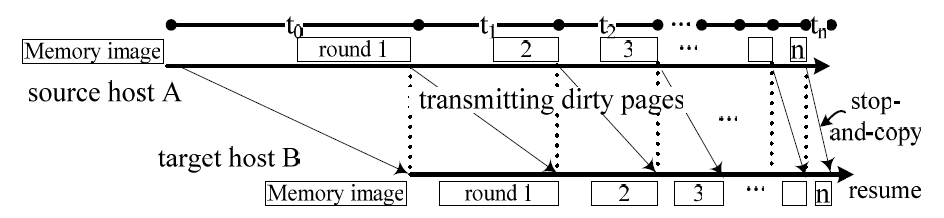
\includegraphics[width=0.7\textwidth]{figures/state_of_the_art/VM_migration_precopy.PNG}
	\caption{Live migration algorithm performs pre-copying in iterative rounds \cite{liu2013performance}}
	\label{fig:VM_migration_precopy}
\end{figure}

The pre-copying phase is terminated when any of the following conditions are satisfied:

\begin{enumerate}
	\item [1)] memory dirtying rate exceeds memory transmission rate
	\item [2)] the remaining dirty memory falls below a predefined threshold
	\item [3)] the number of pre-copying iterations exceeds a defined maximum
	\item [4)] total network traffic exceeds a multiple of the VM memory size
\end{enumerate}

Findings in this work include that with incremental data transmission rate (bandwidth) the power consumption progressively increases while the migration latency decreases. Also, power consumption during migrations increase for both source and destination hosts from which the resulting migration energy can be derived. In addition the migration load and time needed for each pre-copy iteration as well as the total migration load and latency are calculated. 

Besides the defined base model a refined migration model is specified which takes into account the size of a workload's writable working set, that is the number of pages dirtied most frequently. The latter model has been empirically evaluated by measuring the WWS on a Xen virtual machine and deriving the maximum sensible pre-copy iteration while continuously checking termination conditions. 

Workloads with different sizes for writable working sets have been evaluated in simulations including two hosts running 8 virtual machines. 
The resulting migration downtime, migration latency, network traffic and energy consumption could be reduced by 72.9\%, 93.5\%, 74.5\% and 73.6\% compared to a random selection technique, respectively (Figure \ref{fig:vm_migration_normalized_cost}). 

\begin{figure}[htbp]
	\centering
		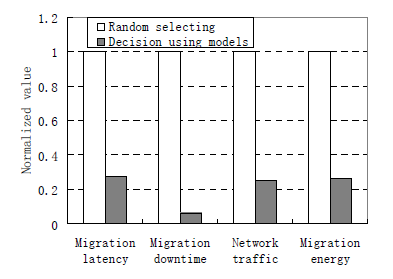
\includegraphics[width=0.5\textwidth]{figures/state_of_the_art/vm_migration_normalized_cost.PNG}
	\caption{Migration cost savings by using proposed models \cite{liu2013performance}}
	\label{fig:vm_migration_normalized_cost}
\end{figure}



%Migration costs and downtime may vary significantly depending on the type of workload and VM configuration parameters. The authors leverage cost prediction schemes to yield expected costs for specific VM migrations. 









%See "`Live Virtual Machine Migration via Asynchronous Replication and State Synchronization"'


%There are different proposed approaches related to virtual machine migration in distributed cloud environments \cite{celesti2010improving, malet2010resource}. In \cite{celesti2010improving} the so-called Composed Image Cloning (CIC) methodology designed for migration of VMs across federated clouds is introduced. This work aims to reduce the needed bandwidth and migration time by setting up a new virtual machine in the destination cloud and transferring only user data instead of relocating the whole VM disc image. 
%
%In another work \cite{malet2010resource} the placement of applications is dynamically adjusted across distributed data centers according to the location of the currently highest request rate. 


